% sections/results.tex — numbers only through \res{}; every claim has a row in paper/CLAIMS.md.
% Draft for the author's review (plan of sections approved 2026-10-18, PLAN §6); revised after the review r1
% (docs/reviews/2026-10-19-q1-manuscript-r1.md): planned outputs added, post hoc descriptions of §12, 2026-10-19 marked.
\section{Results}\label{sec:results}

Every estimate below comes from a registered run and is labelled as confirmatory (a hypothesis of the frozen plan),
secondary, descriptive or post hoc; \ref{app:deviations} lists the deviations from the plan. Gaps $\hat g$ are
normalised by the scale of the reference solution (Section~\ref{sec:metrics}), and the target is $\hat g \le \tau$ with
$\tau = 10^{-3}$.

\subsection{RQ1: the ceiling of the surrogate and the sampler}\label{sec:res-rq1}

RQ1 is studied on pairs of factor instances with $N \in \{16, 24\}$, where the optimum and the best subsets of the
surrogate are certified by enumeration. With a larger dispersion of volatilities (and betas), the ceiling of the
equal-weight surrogate is higher (H1a confirmed, Holm-adjusted $p = \res{e1.h1a.p.holm}$); the direction was expected
from the construction of the surrogate, and the size is the information. By the floor rule of the plan the test is at
$m_0 = \res{e1.h1a.m0}$, the best subset of the surrogate. In \res{e1.h1a.npos} of the \res{e1.h1a.npairs} pairs of
instances the ceiling is higher at the high dispersion, in \res{e1.h1a.nneg} it is lower and in \res{e1.h1a.nzero} the
two tie; the mean difference is \res{e1.h1a.diff.mean} in $\hat g$ (\res{e1.h1a.diff.level.pct}\% CI
\res{e1.h1a.diff.mean.ci.low}--\res{e1.h1a.diff.mean.ci.high}). As estimates: the best surrogate subset misses the
target on \res{e1.eform.m1.h015.pct}\% of the instances at the low dispersion and on \res{e1.eform.m1.h045.pct}\% at
the high one, while an oracle that refines the $m = 50$ best subsets of the surrogate leaves
\res{e1.eform.m50.h015.nexceed} of \res{e1.eform.m50.h015.ninstances} and \res{e1.eform.m50.h045.nexceed} of
\res{e1.eform.m50.h045.ninstances} instances above the target.

Real samplers do not deliver such a pool (Table~\ref{tab:samplers-rq1}; one call of fixed work, about one second).
Single-flip annealing with a penalty misses the best subset of the surrogate on most instances (it finds it within
$\tau$ on \res{e1.samp.sa.m1.within.pct}\% of them), and its pipeline stays above the target on
\res{e1.pipe.sa.m200.nabove} of \res{e1.pipe.ninstances} instances. Tabu search and swap-SA find the best subset on
\res{e1.samp.tabu.m1.within.pct}\% and \res{e1.samp.swap.m1.within.pct}\% of the instances, but one call returns a
median of only \res{e1.pool.tabu.unique} and \res{e1.pool.swap.unique} distinct subsets, so that their pipelines stay
above the target on \res{e1.pipe.tabu.m200.nabove} and \res{e1.pipe.swap.m200.nabove} instances, against
\res{e1.eform.m50.all.nexceed} for the oracle pool of 50. A hotter swap-SA (exploratory) returns
\res{e1.pool.swaphot.unique} distinct subsets per call and leaves \res{e1.pipe.swaphot.m200.nabove} instances above the
target: for the pipeline, the diversity of the pool mattered more than the minimisation of the surrogate.

\begin{table}[t]
\centering\footnotesize\setlength{\tabcolsep}{4pt}
\caption{RQ1, real samplers at $N \in \{16, 24\}$ (\res{e1.pipe.ninstances} instances, one call of fixed work): the
share of instances on which the sampler finds the best subset of the surrogate within $\tau$, the median number of
distinct subsets per call, and the instances on which the pipeline (refining the pool, at most 200 subsets) stays
above the target. The oracle pool of the 50 best subsets leaves \res{e1.eform.m50.all.nexceed}.
$^{\S}$Exploratory.}\label{tab:samplers-rq1}
\begin{tabular}{lrrr}
\toprule
Sampler & best subset (\%) & distinct subsets & above target \\
\midrule
SA, penalty & \res{e1.samp.sa.m1.within.pct} & \res{e1.pool.sa.unique} & \res{e1.pipe.sa.m200.nabove} \\
tabu, penalty & \res{e1.samp.tabu.m1.within.pct} & \res{e1.pool.tabu.unique} & \res{e1.pipe.tabu.m200.nabove} \\
swap-SA & \res{e1.samp.swap.m1.within.pct} & \res{e1.pool.swap.unique} & \res{e1.pipe.swap.m200.nabove} \\
swap-SA, hotter$^{\S}$ & \res{e1.samp.swaphot.m1.within.pct} & \res{e1.pool.swaphot.unique} & \res{e1.pipe.swaphot.m200.nabove} \\
\bottomrule
\end{tabular}
\end{table}

The exploratory finding that tabu search beats simulated annealing at an equal budget, whose direction a recent audit
also reports~\cite{lozano2026where}, replicated on the held-out factor family (H1c confirmed, Holm-adjusted
$p = \res{e1.h1c.p.holm}$). H1c runs on the non-trivial instances of C1--C3 at 10~s end-to-end with equal tuning:
tabu search ended lower on \res{e2.h1c.tabubetter} of the \res{e2.h1c.n} instances, never higher
(\res{e2.h1c.sabetter}), and tied on \res{e2.h1c.zero}. The outcome reads more narrowly than its wording
(\ref{app:deviations}): in the frozen tuning space the single-flip annealing is held by the penalty barrier of the
inclusion QUBO and did not improve the common start in any of its runs, so the test counts the instances on which
tabu search improved the start. It shows that tabu search improves the common start where the annealing of the plan
cannot, not that tabu search is better than simulated annealing in general; an exploratory annealing with a smaller
penalty, recorded in the plan, was not run.

\subsection{Most instances of the design need no combinatorial search}\label{sec:res-a3}

The screening of the plan separates the instances on which the common start --- the refined solution of the
continuous relaxation that every method receives --- is already within the target. Their share is large on the
factor instances: \res{e2.a3.c1.pct}\%, \res{e2.a3.c2.pct}\% and \res{e2.a3.c3.pct}\% in C1, C2 and C3
(Figure~\ref{fig:a3}), under the design of these cells ($K$ half the support of the continuous optimum,
$\lambda = 5$, $\tau = 10^{-3}$). It is \res{e2.a3.c4.pct}\% on the S\&P~500 bootstrap (C4) and \res{e2.a3.c5.pct}\%
of the \res{e2.a3.c5.nscanned} OR-Library points on which the cardinality constraint binds (C5; the other
\res{e2.a3.c5.nnonbinding} of the 125 points do not bind). No dense instance of D1 was trivial, but the screening
decided only \res{e2.a3.d1.n100.nnontrivial} of 20 instances at $N = 100$ and \res{e2.a3.d1.n200.nnontrivial} of 20 at
$N = 200$ within its limit; the others remain undetermined. The comparisons of RQ2 use the non-trivial instances only.

What remains to be gained is small on the factor instances. The gap of the common start, in basis points of the
annual certainty equivalent over all screened instances, has a median of \res{e2.a3.c1.gstart.median.bp},
\res{e2.a3.c2.gstart.median.bp} and \res{e2.a3.c3.gstart.median.bp}~bp and a maximum of
\res{e2.a3.c1.gstart.max.bp}, \res{e2.a3.c2.gstart.max.bp} and \res{e2.a3.c3.gstart.max.bp}~bp in C1--C3; the target
itself corresponds to \res{e2.tau.bp.factor}~bp at the median scale of the non-trivial instances of these cells. The S\&P cell is different (median
\res{e2.a3.c4.gstart.median.bp}~bp, maximum \res{e2.a3.c4.gstart.max.bp}~bp). Proving triviality has a cost: the
certificate on the trivial instances took a median of \res{e2.a3.c1.tcert.median}~s in C1 and
\res{e2.a3.c3.tcert.median}~s in C3, with a maximum of \res{e2.a3.c3.tcert.max}~s in C3 and
\res{e2.a3.c5.tcert.max}~s in C5.

\begin{figure}[t]
\centering
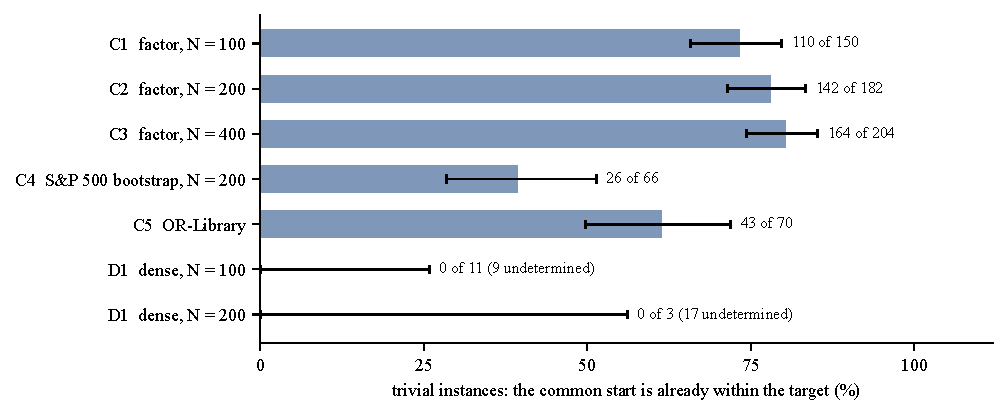
\includegraphics[width=\textwidth]{generated/figures/fig_a3_trivial.pdf}
\caption{Share of trivial test instances by cell: the common start is already within the target
($\hat g \le 10^{-3}$), among the instances the screening decided. Wilson \res{e2.a3.level.pct}\% intervals and
counts; C4 and D1 (dense covariance) are descriptive, and the dense instances the screening left undetermined are
counted apart.}\label{fig:a3}
\end{figure}

\subsection{RQ2: anytime comparison on the non-trivial instances}\label{sec:res-rq2}

The representative of the QUBO class is the tuned winner of the pre-registered tuning, swap-SA, which keeps $K$ assets
by construction and needs no penalty; the penalty samplers of the same runs are reported below. References are
certified optima for all non-trivial instances except \res{e2.c5.uncertified} OR-Library points and the
\res{e2.d1.uncertified} dense ones, where they are the best known values.

\paragraph{Primal integral} Against the open-source exact class, the QUBO pipeline approaches the optimum faster (H2:
pooled $R = \res{e2.h2}$, \res{e2.level.pct}\% CI \res{e2.h2.ci.low}--\res{e2.h2.ci.high}, outcome ``QUBO
better''). The outcome holds without the OR-Library cell (\res{e2.h2.noc5},
\res{e2.h2.noc5.ci.low}--\res{e2.h2.noc5.ci.high}) and when the integral of a method counts from its first
improvement of the common start (\res{e2.h2.firstimpr}); with the integral over $[0, T]$, the measure before the
deviation A2, only its direction is established (\res{e2.h2.full}, \res{e2.h2.full.ci.low}--\res{e2.h2.full.ci.high};
Table~\ref{tab:rq2}). By cell, the advantage is established in C2 and C3, all three OR-Library ports lie on the same
side, and in C1 the data do not distinguish the methods. The comparison is with open-source exact methods only
(Table~\ref{tab:m11}).

Against local search the pooled order is reversed (H2b: $R_b = \res{e2.h2b}$,
\res{e2.h2b.ci.low}--\res{e2.h2b.ci.high}, outcome ``QUBO worse''). This outcome rests on the OR-Library cell, which
has only \res{e2.c5.nports} port clusters, so that its interval is the range of the port means. Without C5 (a post hoc
check) the estimate is \res{e2.h2b.noc5} (\res{e2.h2b.noc5.ci.low}--\res{e2.h2b.noc5.ci.high}), from the first
improvement \res{e2.h2b.firstimpr} (\res{e2.h2b.firstimpr.ci.low}--\res{e2.h2b.firstimpr.ci.high}) and over $[0, T]$
\res{e2.h2b.full} (\res{e2.h2b.full.ci.low}--\res{e2.h2b.full.ci.high}): in each of these variants local search is
faster on average, but the size of the difference relative to the band $[1/1.5, 1.5]$ is not determined. % num-ok: the equivalence band of the plan

The average hides a split over the instances (Table~\ref{tab:rq2-inst}, descriptive and post hoc). On the typical
factor instance the QUBO pipeline is the faster of the two: the median $R_b$ is \res{e2.inst.c1.rb.median},
\res{e2.inst.c2.rb.median} and \res{e2.inst.c3.rb.median} in C1--C3, and $R_b < 1$ on
\res{e2.inst.c1.rb.below.pct}\%, \res{e2.inst.c2.rb.below.pct}\% and \res{e2.inst.c3.rb.below.pct}\% of the
instances. On a minority it fails: the median over its seeds of the time to the target lies beyond the budget on
\res{e2.censor.c1.qubo}, \res{e2.censor.c2.qubo} and \res{e2.censor.c3.qubo} of the 40 instances of C1--C3 and on
\res{e2.censor.c4.qubo} of 40 in C4, and the largest $R_b$ in C1 is \res{e2.inst.c1.rb.max}. The median time to the
target of local search was within the budget on every instance. The geometric mean of the plan weighs these failures, and they decide H2b; on the S\&P and
OR-Library cells local search is also faster on the typical instance (median $R_b$ \res{e2.inst.c4.rb.median} and
\res{e2.inst.c5.rb.median}).

\begin{table}[t]
\centering\small\setlength{\tabcolsep}{4pt}
\caption{RQ2: ratios of the primal integral after the common start, $R = \mathrm{PI}^{+}(\text{QUBO}) /
\mathrm{PI}^{+}(\text{exact})$ and $R_b = \mathrm{PI}^{+}(\text{QUBO}) / \mathrm{PI}^{+}(\text{local search})$; below 1
the QUBO pipeline is better. Cells: estimate and \res{e2.celllevel.pct}\% interval per cell (Bonferroni, simultaneous
99\% over the four pooled cells; for C5 the range of the three port means); $n$ non-trivial instances % num-ok: family level of the plan
(clusters). Pooled rows: \res{e2.level.pct}\% intervals; the last two (post hoc) replace the exact representative by SCIP
with aggressive primal heuristics or by outer approximation in every cell. $^{\dagger}$Descriptive cell, not
pooled.}\label{tab:rq2}
% generated by scripts/paper_tables.py; do not edit by hand.
\begin{tabular}{lrll}
\toprule
Cell & $n$ & $R$ (H2) & $R_b$ (H2b) \\
\midrule
C1 & 40 & 0.447 [0.133, 1.77] & 2.87 [0.864, 11.3] \\
C2 & 40 & 0.0814 [0.0342, 0.229] & 1.47 [0.571, 4.22] \\
C3 & 40 & 0.182 [0.0745, 0.421] & 1.49 [0.712, 3.50] \\
C4$^{\dagger}$ & 40 & 0.723 [0.231, 2.05] & 19.5 [6.28, 54.6] \\
C5 & 27 (3) & 0.109 [0.0292, 0.514] & 7.50 [2.05, 37.1] \\
D1, $N=100$$^{\dagger}$ & 11 & 0.128 [0.0624, 0.304] & 4.15 [1.44, 10.7] \\
D1, $N=200$$^{\dagger}$ & 3 & 0.815 [0.718, 1.000] & 7.28 [4.91, 9.73] \\
\midrule
\multicolumn{2}{l}{Pooled (C1--C3, C5)} & 0.164 [0.106, 0.257] & 2.62 [1.71, 4.08] \\
\midrule
\multicolumn{2}{l}{Without C5 (post hoc)} & 0.188 [0.127, 0.283] & 1.85 [1.26, 2.76] \\
\multicolumn{2}{l}{$\gamma = 1$ until the first improvement} & 0.106 [0.0700, 0.163] & 2.29 [1.42, 3.82] \\
\multicolumn{2}{l}{No common start (cold runs)} & 0.0376 [0.0315, 0.0433] & 0.143 [0.128, 0.167] \\
\multicolumn{2}{l}{PI over $[0, T]$ (with $t_0$)} & 0.738 [0.630, 0.860] & 1.60 [1.34, 2.04] \\
\multicolumn{2}{l}{Exact: SCIP, aggressive heuristics} & 0.108 [0.0703, 0.169] & 2.62 [1.71, 4.08] \\
\multicolumn{2}{l}{Exact: OA in every cell} & 0.128 [0.0783, 0.212] & 2.62 [1.71, 4.08] \\
\bottomrule
\end{tabular}

\end{table}

\begin{table}[t]
\centering\small\setlength{\tabcolsep}{3.5pt}
\caption{RQ2 over the instances (descriptive, post hoc): medians of $R$ and $R_b$, the shares of instances with
ratios below 1, the largest $R_b$, and the instances on which the median time to the target of a method lies beyond
the 60~s budget (target not reached). $^{\dagger}$Descriptive cell.}\label{tab:rq2-inst}
% generated by scripts/paper_tables.py; do not edit by hand.
\begin{tabular}{lrrrrrrrrr}
\toprule
 & & \multicolumn{2}{c}{$R$} & \multicolumn{3}{c}{$R_b$} & \multicolumn{3}{c}{target not reached} \\
\cmidrule(lr){3-4}\cmidrule(lr){5-7}\cmidrule(lr){8-10}
Cell & $n$ & median & $<1$ (\%) & median & $<1$ (\%) & max & QUBO & LS & exact \\
\midrule
C1 & 40 & 0.12 & 62 & 0.79 & 57 & 378 & 6 & 0 & 0 \\
C2 & 40 & 0.026 & 80 & 0.47 & 68 & 81 & 2 & 0 & 0 \\
C3 & 40 & 0.19 & 82 & 0.66 & 57 & 100 & 4 & 0 & 6 \\
C4$^{\dagger}$ & 40 & 2.4 & 38 & 73 & 25 & 249 & 24 & 0 & 0 \\
C5 & 27 & 0.23 & 78 & 10.0 & 22 & 293 & 6 & 0 & 9 \\
D1, $N=100$$^{\dagger}$ & 11 & 0.100 & 100 & 4.0 & 18 & 19 & 1 & 0 & 3 \\
D1, $N=200$$^{\dagger}$ & 3 & 0.75 & 100 & 8.1 & 0 & 9.7 & 3 & 0 & 3 \\
\bottomrule
\end{tabular}

\end{table}

\paragraph{Penalty samplers} With the tuned penalty samplers of the same runs in the place of the representative
(post hoc, Table~\ref{tab:samplers}), the QUBO pipeline is slower than the open-source exact class --- single-flip
annealing $R = \res{e2.sa.h2}$ (\res{e2.sa.h2.ci.low}--\res{e2.sa.h2.ci.high}), tabu search $R = \res{e2.tabu.h2}$
(\res{e2.tabu.h2.ci.low}--\res{e2.tabu.h2.ci.high}) --- and far slower than local search ($R_b = \res{e2.sa.h2b}$ and
\res{e2.tabu.h2b}). In this benchmark the advantage of H2 belongs to the sampler that preserves the cardinality, not to
the penalty samplers.

\begin{table}[t]
\centering\footnotesize\setlength{\tabcolsep}{3pt}
\caption{RQ2 with other QUBO samplers (post hoc): the same estimator with the tuned single-flip annealing (SA) and tabu
search of the same runs, both on the penalty QUBO, in the place of the representative swap-SA; cell estimates and the
pooled estimates over C1--C3 and C5 with \res{e2.level.pct}\% intervals. $^{\dagger}$Descriptive cell.}\label{tab:samplers}
% generated by scripts/paper_tables.py; do not edit by hand.
\begin{tabular}{lllllll}
\toprule
 & \multicolumn{3}{c}{$R$ (against the exact class)} & \multicolumn{3}{c}{$R_b$ (against local search)} \\
\cmidrule(lr){2-4}\cmidrule(lr){5-7}
Cell & swap-SA & SA & tabu & swap-SA & SA & tabu \\
\midrule
C1 & 0.447 & 37.3 & 14.5 & 2.87 & 240 & 93.2 \\
C2 & 0.0814 & 6.06 & 1.55 & 1.47 & 109 & 28.0 \\
C3 & 0.182 & 5.28 & 1.62 & 1.49 & 43.3 & 13.3 \\
C4$^{\dagger}$ & 0.723 & 5.22 & 3.77 & 19.5 & 141 & 102 \\
C5 & 0.109 & 3.02 & 3.02 & 7.50 & 207 & 207 \\
\midrule
Pooled & 0.164 & 7.74 & 3.24 & 2.62 & 124 & 51.7 \\
95\% CI & [0.106, 0.257] & [6.81, 8.79] & [2.56, 4.04] & [1.71, 4.08] & [116, 132] & [41.4, 64.1] \\
\bottomrule
\end{tabular}

\end{table}

\paragraph{The common start decides the order of H2b} Without the common start (cold runs, a sensitivity of the plan)
the order of H2b reverses: $R_b = \res{e2.h2b.own}$ (\res{e2.h2b.own.ci.low}--\res{e2.h2b.own.ci.high}). The reason is
the time to a method's first own portfolio (Table~\ref{tab:exact}): the QUBO pipeline holds one after its first batch
(medians from \res{e2.delay.c1.qubo.median}~s in C1 to \res{e2.delay.c3.qubo.median}~s in C3), local search only when
its greedy construction ends (\res{e2.delay.c1.ls.median}~s to \res{e2.delay.c3.ls.median}~s), and the exact
representative after \res{e2.delay.c1.exact.median}~s to \res{e2.delay.c3.exact.median}~s. The common start itself
is ready earlier still (medians from \res{e2.t0.c1.median}~s in C1 to \res{e2.t0.c3.median}~s in C3), and in the
cold runs no method held its first portfolio before that time on any instance (post hoc). The first portfolio of the
QUBO pipeline was at least as good as the common start on \res{e2.first.c1.qubo.notworse.pct}\%,
\res{e2.first.c2.qubo.notworse.pct}\% and \res{e2.first.c3.qubo.notworse.pct}\% of the instances of C1--C3, that of
local search on \res{e2.first.c1.ls.notworse.pct}\%, \res{e2.first.c2.ls.notworse.pct}\% and
\res{e2.first.c3.ls.notworse.pct}\%. With the common start, the start covers this interval for every method.

\begin{table}[t]
\centering\small
\caption{The exact class by cell (secondary): the exact representative, the median time of its last improvement
$t_{\mathrm{primal}}$ and the share of its runs certified within the 60~s budget; and the median delay to the first
own solution of each representative in the cold runs (no common start). $^{\dagger}$Descriptive cell.}\label{tab:exact}
% generated by scripts/paper_tables.py; do not edit by hand.
\begin{tabular}{llrrrrr}
\toprule
Cell & exact method & $t_{\mathrm{primal}}$ (s) & certified (\%) & \multicolumn{3}{c}{first own solution (s)} \\
\cmidrule(lr){5-7}
 & & & & QUBO & LS & exact \\
\midrule
C1 & SCIP & 1.5 & 100 & 0.064 & 0.59 & 0.55 \\
C2 & SCIP & 8.6 & 72 & 0.19 & 1.6 & 3.9 \\
C3 & OA (HiGHS) & 7.5 & 18 & 0.57 & 3.7 & 7.4 \\
C4$^{\dagger}$ & SCIP & 12 & 68 & 0.19 & 1.2 & 3.9 \\
C5 & SCIP & 15 & 7 & 0.067 & 0.79 & 0.50 \\
\bottomrule
\end{tabular}

\end{table}

\paragraph{Time to target} The time to the target gives the same pooled outcomes (secondary): QUBO over exact
\res{e2.ttt} (\res{e2.ttt.ci.low}--\res{e2.ttt.ci.high}) and QUBO over local search \res{e2.tttb}
(\res{e2.tttb.ci.low}--\res{e2.tttb.ci.high}); re-censored at 10~s, the second weakens to a direction
(\res{e2.tttb.budget10}, \res{e2.tttb.budget10.ci.low}--\res{e2.tttb.budget10.ci.high}). By the performance profiles
at ratio 1~\cite{dolan2002benchmarking}, the QUBO pipeline has the smallest integral on \res{e2.profile.pi.c1.qubo.pct}\%,
\res{e2.profile.pi.c2.qubo.pct}\% and \res{e2.profile.pi.c3.qubo.pct}\% of the instances of C1, C2 and C3, local search
on \res{e2.profile.pi.c4.ls.pct}\% and \res{e2.profile.pi.c5.ls.pct}\% of C4 and C5. The exact representative
certifies the optimum within the budget in \res{e2.exact.c1.cert.pct}\% of its runs in C1, \res{e2.exact.c2.cert.pct}\%
in C2, \res{e2.exact.c3.cert.pct}\% in C3 and \res{e2.exact.c5.cert.pct}\% in C5.

The time-to-target curves~\cite{aiex2006ttt} on three calibration instances of $N = 200$ (100 runs per method,
Figure~\ref{fig:ttt}, descriptive) illustrate the split. Local search reaches the target in every run on all three
instances (medians \res{e2.curves.1014.ls.median}, \res{e2.curves.1043.ls.median} and
\res{e2.curves.1049.ls.median}~s), the exact representative in \res{e2.curves.1014.exact.pct}\%,
\res{e2.curves.1043.exact.pct}\% and \res{e2.curves.1049.exact.pct}\% of its runs (medians
\res{e2.curves.1014.exact.median}, \res{e2.curves.1043.exact.median} and \res{e2.curves.1049.exact.median}~s). The QUBO
pipeline is the fastest method on the first instance (median \res{e2.curves.1014.qubo.median}~s), behind local search
on the second (\res{e2.curves.1043.qubo.median}~s), and never reaches the target within 60~s on the third
(\res{e2.curves.1049.qubo.pct}\% of the runs). These instances were also used for tuning; the counts of
Table~\ref{tab:rq2-inst} come from the test instances.

\begin{figure}[t]
\centering
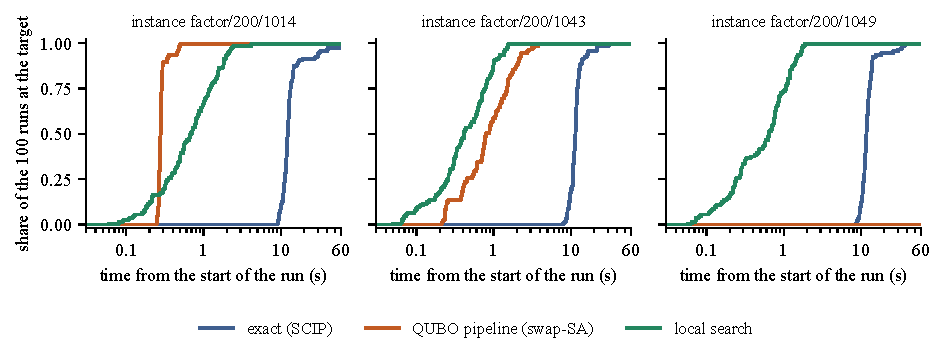
\includegraphics[width=\textwidth]{generated/figures/fig_ttt_curves.pdf}
\caption{Time-to-target curves ($\hat g \le 10^{-3}$) of the three representatives on three calibration instances of
$N = 200$: the share of 100 runs at the target against the time from the start of the run (log scale). Runs that miss
the target stay in the denominator.}\label{fig:ttt}
\end{figure}

\paragraph{The exact baseline}\label{sec:res-m11} The representative of the exact class was chosen by the tuning
criterion, the median $\mathrm{PI}^{+}$ on the calibration instances. At $N = 200$ outer approximation won the 10~s
screen (\res{e2.tune.n200.oa.screen} against \res{e2.tune.n200.scip.screen} for SCIP) but lost the 60~s recheck
(\res{e2.tune.n200.oa.long} against \res{e2.tune.n200.scip.long}), so SCIP is the representative at $N = 100$ and 200
and outer approximation at $N = 400$. On problem~(34) of Bertsimas and Cory-Wright~\cite{bertsimas2022scalable} and
the times of their Tables~3 and~4 (arXiv version~5; BCW-T3 and BCW-T4 below), SCIP needed in the median
\res{e2.m11.t3.scip.median} times the best published time on BCW-T3 and \res{e2.m11.t4.scip.median} times on BCW-T4
(Table~\ref{tab:m11}, Figure~\ref{fig:m11}); outer approximation needed \res{e2.m11.t3.oa.median} times on BCW-T3.
The best published times on BCW-T3 are a few hundredths of a second (median \res{e2.m11.t3.pub.time.median}~s,
printed to two decimals), against a median of \res{e2.m11.t3.scip.time.median}~s for SCIP, including the build of
the model in Python. On BCW-T4 SCIP solved all \res{e2.m11.t4.scip.ncells} instances within the limit, the best
published method \res{e2.m11.t4.scip.npub}, and SCIP was faster on \res{e2.m11.t4.scip.nfaster} of them
(\res{e2.m11.t4.scip.faster.cells}). The times are not normalised for the hardware, and the validation measures the
time to a certificate, not the speed of improvement that H2 measures. By the rule of the plan (a median ratio above
10), the conclusions of RQ2 concern open-source exact methods, and the outcome of H2 carries this caveat.

Two post hoc runs re-solved the same non-trivial instances with other open-source exact baselines (\ref{app:deviations},
19 October; Table~\ref{tab:rq2}): SCIP in the configuration of the representative with its aggressive primal
heuristics, and outer approximation as the representative in every cell. The pooled ratio stays below the band in
both, $R = \res{e2.exactsens.scipaggr.h2}$ (\res{e2.exactsens.scipaggr.h2.ci.low}--\res{e2.exactsens.scipaggr.h2.ci.high})
and $R = \res{e2.exactsens.oa.h2}$ (\res{e2.exactsens.oa.h2.ci.low}--\res{e2.exactsens.oa.h2.ci.high}), so the outcome
of H2 does not depend on these choices of the open-source baseline. The aggressive heuristics did not make SCIP improve
its incumbent faster on the factor and S\&P cells: the median ratio of its primal integral to that of the default
setting was \res{e2.exactsens.scipaggr.pirel.c1} in C1, \res{e2.exactsens.scipaggr.pirel.c2} in C2 and
\res{e2.exactsens.scipaggr.pirel.c4} in C4, against \res{e2.exactsens.scipaggr.pirel.c5} on the OR-Library points.

\begin{table}[t]
\centering\small\setlength{\tabcolsep}{4pt}
\caption{Validation of the exact stack against Tables~3 ($\kappa = 1$, limit 300~s) and~4 ($\kappa = 0$ with a
minimum return, limit 3600~s) of Bertsimas and Cory-Wright (BCW-T3, BCW-T4): the median over the 15 instances of each
table of our time over the best published time (SCIP gives the verdict; outer approximation and the better of our
two methods for reference), the median times, and the instances solved within the limit.}\label{tab:m11}
% generated by scripts/paper_tables.py; do not edit by hand.
\begin{tabular}{lrrrrrrr}
\toprule
 & \multicolumn{3}{c}{median ratio} & \multicolumn{2}{c}{median time (s)} & \multicolumn{2}{c}{solved} \\
\cmidrule(lr){2-4}\cmidrule(lr){5-6}\cmidrule(lr){7-8}
BCW table & SCIP & OA & best of ours & SCIP & BCW best & ours & BCW \\
\midrule
BCW-T3 & 262 & 3.1 & 3.1 & 4.9 & 0.020 & 15/15 & 15/15 \\
BCW-T4 & 14 & -- & 14 & 651 & 21 & 15/15 & 14/15 \\
\bottomrule
\end{tabular}

\end{table}

\begin{figure}[t]
\centering
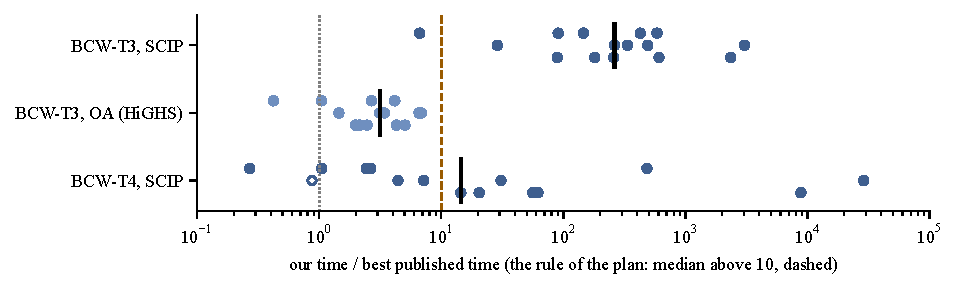
\includegraphics[width=\textwidth]{generated/figures/fig_m11_ratios.pdf}
\caption{Ratio of our time to the best published time per instance (dots, three cardinalities per port) and their
median (bar). Hollow: every published method hit the limit, so the ratio is an upper bound.}\label{fig:m11}
\end{figure}

\subsection{RQ3: does optimisation accuracy matter out of sample?}\label{sec:res-rq3}

On FF49 the cardinality constraint binds on \res{e3.ff.binding.pct}\% of the walk-forward folds (median
$K = \res{e3.ff.k.median}$), and the lower bound of the rule for $K$ is active on \res{e3.ff.regime.lb.pct}\% of them
(\res{e3.us.regime.lb.pct}\% on the US universe): with $K u$ close to one, the weights are nearly fixed and the
alternatives differ mainly in which assets (on FF49, industries) they hold. The best non-optimal support (rank 2) is close to the
optimum in sample: its gap has a median of \res{e3.ff.mv.dose2.median}~bp of certainty equivalent per year for the
mean--variance arm, \res{e3.ff.gmv.dose2.median}~bp for the minimum-variance arm and \res{e3.us.mv.dose2.median}~bp on
the US universe (Table~\ref{tab:rq3-extra}).

For the minimum-variance arm, the rank-2 portfolio and the optimum are equivalent out of sample: the log variance
ratio is \res{e3.ff.gmv.h3a} (\res{e3.h3a.level.pct}\% CI \res{e3.ff.gmv.h3a.ci.low}--\res{e3.ff.gmv.h3a.ci.high})
inside its margin (Holm-adjusted $p_{\mathrm{TOST}} = \res{e3.ff.gmv.h3a.p.tost.holm}$). For the mean--variance arm
(primary) the difference of Sharpe ratios before costs is \res{e3.ff.mv.h3a}
(\res{e3.ff.mv.h3a.ci.low}--\res{e3.ff.mv.h3a.ci.high}) against the margin $\pm\res{e3.ff.mv.margin.high}$:
inconclusive, which is uncertainty and not evidence that accuracy matters. On the US universe the result is also
inconclusive (\res{e3.us.mv.h3a}, \res{e3.us.mv.h3a.ci.low}--\res{e3.us.mv.h3a.ci.high}; Table~\ref{tab:rq3}). These
statements concern the best alternatives, which are close to the optimum by construction, not an error of the same size
in an arbitrary direction.

The sensitivities of the plan leave these outcomes in place: with block lengths of 21 and 63 days instead of the
calibrated ones (\res{e3.ff.mv.block}, \res{e3.ff.gmv.block} and \res{e3.us.mv.block} days) and with execution one day
later the outcomes do not change, nor do they on the US universe with terminal returns of $-30\%$ and $-100\%$ for % num-ok: sensitivity levels of the plan
delisted stocks or on the \res{e3.us.mv.sens.coverage.nfolds} folds on which at least 90\% of the index members have % num-ok: coverage threshold of the plan
usable prices; with the wider margin $\Delta_{\mathrm{SR}} = 0.05$ the mean--variance arm on FF49 % num-ok: sensitivity margin of the plan
becomes equivalent ($p_{\mathrm{TOST}} = \res{e3.ff.mv.sens.dsr005.p.tost}$), on the US universe it does not
($p_{\mathrm{TOST}} = \res{e3.us.mv.sens.dsr005.p.tost}$). After costs of 10~bp per unit of traded notional, the % num-ok: cost level of the plan
difference of Sharpe ratios of the rank-2 path is \res{e3.ff.mv.net10}
(\res{e3.ff.mv.net10.ci.low}--\res{e3.ff.mv.net10.ci.high}) for the mean--variance arm on FF49
(Table~\ref{tab:rq3-extra}).

Along the series of the best alternative supports (H3b, Figure~\ref{fig:dose}), no relation between the in-sample
gap and the out-of-sample Sharpe ratio before costs is detected at this power for the mean--variance arm (slope
\res{e3.ff.mv.h3b.slope} per unit of the logarithm of the dose, \res{e3.h3b.level.pct}\% CI
\res{e3.ff.mv.h3b.slope.ci.low}--\res{e3.ff.mv.h3b.slope.ci.high}); the pointwise interval of the path of rank 5
excludes zero (\res{e3.ff.mv.rank5}, \res{e3.ff.mv.rank5.ci.low}--\res{e3.ff.mv.rank5.ci.high}), one of six
unadjusted intervals. For the minimum-variance arm the relation is significant: a doubling of the mean in-sample dose
raises the out-of-sample variance by \res{e3.ff.gmv.h3b.doubling.pct}\%
(\res{e3.ff.gmv.h3b.doubling.pct.ci.low}--\res{e3.ff.gmv.h3b.doubling.pct.ci.high}\%). H3c is descriptive:
\res{e3.ff.mv.h3c.nmaterial} of the \res{e3.ff.mv.h3c.nsolvers} real solvers leave a material in-sample gap on FF49,
so their calibration against the curve was not tested.

\begin{table}[t]
\centering\footnotesize\setlength{\tabcolsep}{3pt}
\caption{RQ3, H3a (FF49 primary, US secondary): the rank-2 path against the optimum out of sample, as the
difference of Sharpe ratios before costs (MV) or the log variance ratio (GMV); TOST with \res{e3.h3a.level.pct}\%
intervals and the equivalence margins of the plan; $^{*}$Holm-adjusted. $^{\ddagger}$Without the days with irregular
adjustments (sensitivity).}\label{tab:rq3}
% generated by scripts/paper_tables.py; do not edit by hand.
\begin{tabular}{lllll}
\toprule
Market, arm & estimate [90\% CI] & margin & $p_{\mathrm{TOST}}$ & outcome \\
\midrule
FF49, MV & 0.00364 [\ensuremath{-}0.0286, 0.0359] & $\pm$0.0208 & 0.19 & inconclusive \\
FF49, GMV & \ensuremath{-}0.000762 [\ensuremath{-}0.0137, 0.0122] & [\ensuremath{-}0.0417, 0.0400] & \ensuremath{2.0\times10^{-4}}$^{*}$ & equivalent \\
US, MV & \ensuremath{-}0.0183 [\ensuremath{-}0.0765, 0.0399] & $\pm$0.0208 & 0.47$^{*}$ & inconclusive \\
US, MV$^{\ddagger}$ & \ensuremath{-}0.0486 [\ensuremath{-}0.112, 0.0143] & $\pm$0.0208 & 1.0 & inconclusive \\
\bottomrule
\end{tabular}

\end{table}

\begin{table}[t]
\centering\footnotesize\setlength{\tabcolsep}{2.5pt}
\caption{RQ3, the context of H3a: the in-sample gap of the rank-2 path (bp of certainty equivalent per year, median and
interquartile range over the folds) and the difference of Sharpe ratios of the rank-2 path against the optimum after
costs of 10~bp (main) and 30~bp per unit of traded notional, with 95\% intervals.}\label{tab:rq3-extra} % num-ok: cost levels and confidence level of the plan
% generated by scripts/paper_tables.py; do not edit by hand.
\begin{tabular}{llll}
\toprule
Market, arm & dose of rank 2 (bp) & \multicolumn{2}{c}{$\Delta$Sharpe after costs [95\% CI]} \\
\cmidrule(lr){3-4}
 & median [IQR] & 10~bp & 30~bp \\
\midrule
FF49, MV & 6.1 [2.3, 13] & \ensuremath{-}0.0020 [\ensuremath{-}0.041, 0.037] & \ensuremath{-}0.013 [\ensuremath{-}0.052, 0.025] \\
FF49, GMV & 3.3 [1.5, 6.7] & 0.032 [\ensuremath{-}0.013, 0.076] & 0.020 [\ensuremath{-}0.026, 0.064] \\
US, MV & 2.7 [0.93, 7.2] & \ensuremath{-}0.021 [\ensuremath{-}0.092, 0.049] & \ensuremath{-}0.025 [\ensuremath{-}0.097, 0.046] \\
\bottomrule
\end{tabular}

\end{table}

\begin{figure}[t]
\centering
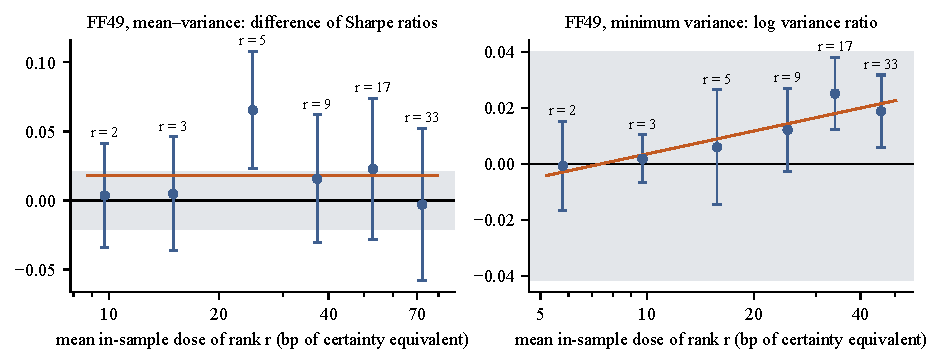
\includegraphics[width=\textwidth]{generated/figures/fig_rq3_dose.pdf}
\caption{FF49: the out-of-sample difference of the path that holds the support of rank $r$ against the optimum, by its
mean in-sample dose, with pointwise \res{e3.h3b.level.pct}\% intervals, the fitted H3b line and the equivalence margin
(grey).}\label{fig:dose}
\end{figure}
